  \section{Enriching the \oeis with a Theory Graph} \label{sec:Enrich}

In the proceeding subsections we first propose a way of representing the \oeis Theory Graph. Then, we discuss an
approach of finding views and discuss the results we get from it.

\subsection{Representing \oeis in Theory Graph} \label{sec:Representation}

First, we need to define the \emph{theory} in the context of \oeis, hence we need to define all the notions related
to the \emph{theory} in this context. We propose the following way to define the theory of a sequence.\\
A sequence $S$ has a corresponding theory which has a typed symbol, $S : nat \mapsto int$ to represent the function
symbol and all the functions are expressed as axioms. Assuming the sequence $S$ contains two functions $f(n)$ and $g
(n)$ the axioms would be:
\begin{equation}
\begin{split}
S_{f}: S &= \lambda n. \ f(n) \\
S_{g}: S &= \lambda n. \ g(n)
\end{split}
\end{equation}

%Where $[n]\ g\ n$ is the equivalent of $\lambda n.gn$.

Now that we have a way to define the theory, we will show  the other notions related to it. The theory inclusions are
 practically the same as in other contexts. The theory $T_i$ that includes theory $T_j$ imports all the symbols of
 theory $T_j$ and they become available in theory $T_i$. An implication of this theory representation is that we can
 represent relations between sequences as views between their corresponding theories.\\
Assume that we have two sequences $S_i$ and $S_j$ and that their respective theories are $T_i$ and $T_j$. If their
corresponding functions are $f$ and $g$, respectively, then theory $T_i$ and $T_j$ can be represented as:\\

\[ T_i = \begin{cases} S_i : nat \mapsto int \\ S_{f} : S_i = f   \\
\end{cases} \]  and
\[ T_j = \begin{cases} S_j : nat \mapsto int \\ S_{g} : S_j = g   \\
\end{cases} \]


If $f$ and $g$ are related through a function $h : (nat \mapsto int) \mapsto (nat \mapsto int)$ such that, $f = h(g)$
 then one can construct a view $\phi$ from $T_i$ to $T_j$, and that is:

\begin{equation}
\phi = \begin{bmatrix} S_i \mapsto h\ S_j  \\ S_{f} \mapsto  \text{proof that the axiom holds in } T_j \end{bmatrix}
\end{equation}

One can easily construct the proof given that we know the function $h$.

A more general case is when the relation occurs between two functions of different sequences but one of the sequences
 has more than one representing function.
Let $S_i$ be a sequence which has $m$ functions and the corresponding theory $T_i$. Since all the functions represent
 the same sequence then they must be equal. We take these as theorems stating the equality of the $m$ functions with
 each other. These are then contained in a special theory $U$, included by all the corresponding theories of sequences. \\
To show this general case, let us have the sequence $S_i$ as above, and a sequence $S_j$ with $k$ functions. Let
there be a relation $h: (nat \mapsto int) \mapsto (nat \mapsto int)$ that maps one of the functions of $S_j$, say
$g_1$ to function $f$ from $S_i$. A view $\theta$, from $T_i$ to $T_j$ needs to have proofs for all the axioms of
$T_i$ under the symbol assignments in $\theta$. The symbol assignment is the same as in the case when $S_j$ had only
one function. From the available theorems in theory $U$ we get $g_1=g_2=...=g_k$. Thus, from $f=h(g_1)$ we get $f=h
(g_i)$ for $i$ in $\{1,\ldots, k\}$, which simplifies the matter to the already explained initial case.
We can encode similarly the case when the view is based on the generating functions.

\subsection{Algorithm}

The current representation of the library allows us to access the formulas present in the \oeis documents. Although
the representing functions are available, we do relation searching on the level of the ordinary generating functions.
 The approach we follow is mathematically simple. We will show three methods, each building on top of the previous one.

\paragraph{Method 1} In this case, we \emph{normalize} the ordinary generating functions of the sequences and check
for equality between the normalized expressions.
The normalization rules are defined as follows:

    \begin{prooftree}
    \AxiomC{$cG$ \ \ \ $c$ - constant \ \ \ $G$ - generating function}
    \RightLabel{\rulename{Const}}
    \UnaryInfC{$G$}
    \end{prooftree}

    \begin{prooftree}
    \AxiomC{$x^nG$ \ \ \ $x$ - the indeterminate of $G$ \ \ \ $G$ - generating function}
    \RightLabel{$\rulename{Unshift}_n$}
    \UnaryInfC{$G$}
    \end{prooftree}

    \begin{prooftree}
    \AxiomC{$P/Q$ \ \ \ $P,Q$ - polynomials}
    \RightLabel{\rulename{Sort}}
    \UnaryInfC{($\sum_{i=0}^{n} p_ix^i) / (\sum_{i=1}^{m} q_ix^i)$ \ \ \ $p_n > 0$ \ \ \ $q_n > 0$}
    \end{prooftree}

The rules are composed in the same order as defined above to form the method \emph{normalize}.
The first two rules are self-evident in what they are supposed to achieve. Rule \rulename{Sort} is used for sorting
the polynomials based on ascending powers of $x$. We add an extra condition on the sign of the highest degree term to
 normalize the sign of the polynomial.

The normalization rules entail easily interpretable relations with the pre-normalized formula. Rule \rulename{Const}
is removing the multiplying constant. Multiplying an ordinary generating function by a constant is equivalent to
multiplying each term of the sequence by that number.
Since multiplying by $x^n$ is the same as shifting the sequence the \rulename{Unshift}$_n$ is normalizing the shift.

Let $B$ (before) be the pre-normalized ordinary generating function, and $A$ (after) the normalized one. Also, let
$\hat{B}(n), \hat{A}(n)$ be the representing functions of the sequence represented by $B,A$, respectively. Then, the
relations that the normalizing rules entail are:

\begin{enumerate}
\item Rule \rulename{Const}: $\hat{A}(n) = \frac{1}{c}\hat{B}(n)$.
\item Rule \rulename{Unshift}$_k$: $\hat{A}(n) = \hat{B}(n+k)$ given that $x^k$ was removed.
\item Rule \rulename{Sort}: $\hat{A}(n) = \hat{B}(n)$.
\end{enumerate}

Intuitively, in this case we are checking if sequences are scaled and/or shifted versions of each other. These
relations are not meant to be interesting or new.

\paragraph{Method 2} In this case we check if a sequence can be expressed as a sum of other sequences existing in the
 \oeis, possibly \emph{normalized} and \emph{transformed}.

A simplified algorithm roughly follows this pseudocode:
\newpage
\begin{lstlisting}[style=myScalastyle]
foreach sequence
    foreach ogf in ordinaryGeneratingFunction(sequence)
        hashSet.put(normalize(ogf))

foreach sequence
    foreach ogf in ordinaryGeneratingFunction(sequence)
        pdf = partialFractionDecomposition(ogf)
        partialFractions = decompose(partialFractions(pfd))
        relationsExists =
            forall pgf in partialFractions
                transformedPartialFractions = normalize(applyTransformations(pgf))
                transformedPartialFractions.intersection(hashSet).nonEmpty
        if (relationsExists)
            print relations
\end{lstlisting}

We will now explain the functions that we are using above.


\begin{wrapfigure}{r}{0pt}
\begin{tikzpicture}[framed]
\node[draw, circle]      (Ti)        {$A_1$};
\node[draw, circle]      (Tj)       [right=of Ti] {$A_2$};
%Lines
\draw[dashed, latex-] (Tj.west) -- (Ti.east);
\end{tikzpicture}
\caption{Relations of \emph{Method 2}}\label{fig:directRelations}
\end{wrapfigure}

Let $GF_n$ be one of the ordinary generating functions of sequence $A_n$. The partial fraction decomposition
(\emph{partialFractionDecomposition}) applied on an ordinary generating function would leave us with:

\begin{equation}
 GF_n = \sum_{j=1}^{n} G_j \label{eq:pfd}
\end{equation}
where $G_j$ is also an ordinary generating function. The function \emph{partialFractions} then takes that sum and
extracts the summands, in this case, the partial fractions (ordinary generating functions) $G_j$. The function
\emph{decompose} does a further step of decomposition. If $G_j = \frac{P}{Q}$ where $P,Q$ are polynomials ( $P =
\sum_{i=0}^{n} a_ix^i$) then it rewrites $G_j = \sum_{i=0}^{n} \frac{a_ix^i}{Q}$. These summands are then considered
'partial fractions', too.

\begin{wrapfigure}{r}{2.8cm}
\begin{tikzpicture}[framed]
\node[draw, circle]      (T)                              {$N$};
\node[draw, circle]        (Tj)       [right=of T] {$A_1$};
\node[draw, circle]      (Ti)       [below=of T] {$A_2$};

%Lines
\draw[latex-] (Ti.north) -- (T.south);
\draw[latex-] (Tj.west) -- (T.east);
\draw[dashed, latex-] (Tj.south) -- (Ti.east);
\end{tikzpicture}
\caption{Relations of \emph{Method 3}}\label{fig:transitiveRelations}
\end{wrapfigure}


The transformations are \emph{integration, differentiation} and \emph{unit}.
The transformations are selected such that expressions that match under these transformations can be easily related
both mathematically and semantically.

Similarly, let $B$ be the pre-transformed ordinary generating function, and $A$ the transformed one. Let $\hat{B}(n),
 \hat{A}(n)$ be the representing function of the sequence represented by $B,A$, respectively. Then, the relations
 that the transformation rules entail are:

\begin{enumerate}
\item Integration: $\hat{A}(n) = \frac{1}{n}\hat{B}(n-1)$.
\item Differentiation: $\hat{A}(n) = n\hat{B}(n+1)$.
\item Unit: $\hat{A}(n) = \hat{B}(n)$.
\end{enumerate}

If $GF_n$ is the ordinary generating function of sequence $A_n$, $c_i$ a real constant, $p \in \{-1,0,1\}$ and $k_i$
an integer, the algorithm would try to find relations of the form:
\begin{equation}
A_j(n) = \sum_{i=0}^{n} c_i n^p A_i(n-k_i)
\end{equation}

In this case we will be finding what we call \emph{direct relations}. So there is a direct \emph{view} between the
sequences (Fig. \ref{fig:directRelations}).


\paragraph{Method 3}

In this case we do not restrict the generating functions to be representing existing \oeis sequences. Instead, we
search if two ordinary generating functions have a common partial fraction in their summation of partial fractions
(Fig. \ref{fig:transitiveRelations}).


% \newpage
The simplified algorithm is given by the pseudocode below.
\begin{lstlisting}[style=myScalastyle]
foreach sequence
    foreach ogf in ordinaryGeneratingFunction(sequence)
        pfd = partialFractionDecomposition(ogf)
        partialFractions = decompose(partialFractions(pfd))
        foreach pgf in partialFraction
            transformations = normalize(applyTransformations(pgf))
            foreach transformed in transformations
                if transformed exists in hashSet
                    print relation
                else
                    add pgf to hashSet
\end{lstlisting}

As an example, let us take two sequences $A_1$ and $A_2$ and their corresponding ordinary generating functions $GF_1$
 and $GF_2$. Let $N$ be a partial fraction and $M,S$ sums of partial fractions. Moreover, for any $G$, if $G$ is an
 ordinary generating function, let $\hat{G}$ denote the representing function of the same sequence that $G$ represents. If
\begin{align}
GF_1 &= M + \int N \\
GF_2 &= S + N
\end{align}
then from the relations defined above and assuming that the representing functions exist, we can carry over the
relation to the representing functions:
\begin{align}
\hat{GF_1}(n) &= \hat{M}(n) + \frac{1}{n}\hat{N}(n-1) \\
\hat{GF_2}(n) &= \hat{S}(n) + \hat{N}(n)
\end{align}
Which then can be solved to give:
\begin{align}
\hat{GF_2}(n) = \hat{S}(n) + (n+1)(\hat{GF_1}(n+1) - \hat{M}(n+1)) \label{eq:transform}
\end{align}

Notice that the step of carrying over the relation between generating functions, to the corresponding representing
functions assumes that the representing functions exist, which is not always the case. Nonetheless, it is worth
noticing that the last equation is independent of $\hat{N}$.

\subsection{Implementation and Evaluation}

\begin{figure}[!h]
\begin{subfigure}{0.3\textwidth}
\centerline{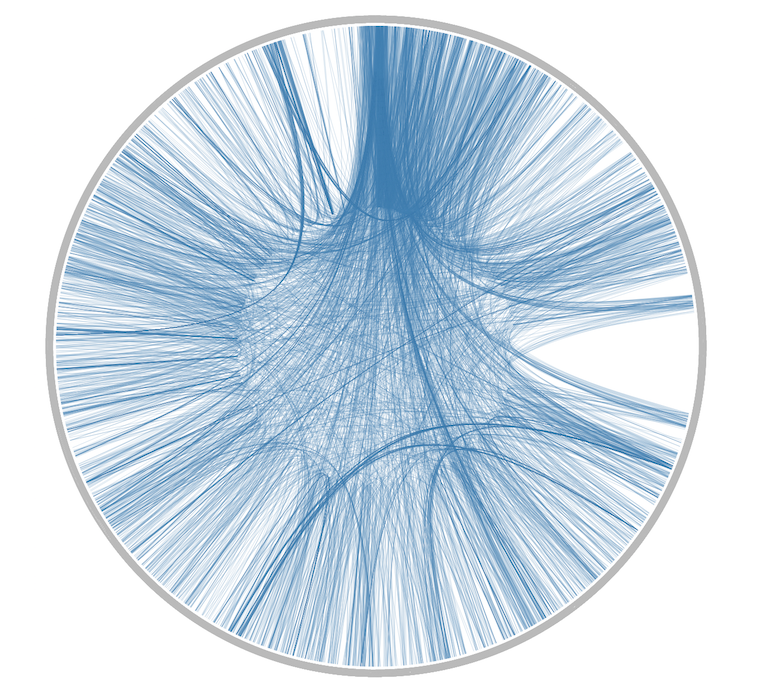
\includegraphics[scale=0.2]{before}}
\caption{OEIS Theory Graph of Explicit Views \label{fig:before}}
\end{subfigure}
\begin{subfigure}{0.3\textwidth}
\centerline{
\includegraphics[scale=0.22]{after}}
\caption{OEIS Theory Graph of Inferred Views using Method 3 \label{fig:after}}
\end{subfigure}
\begin{subfigure}{0.3\textwidth}
\centerline{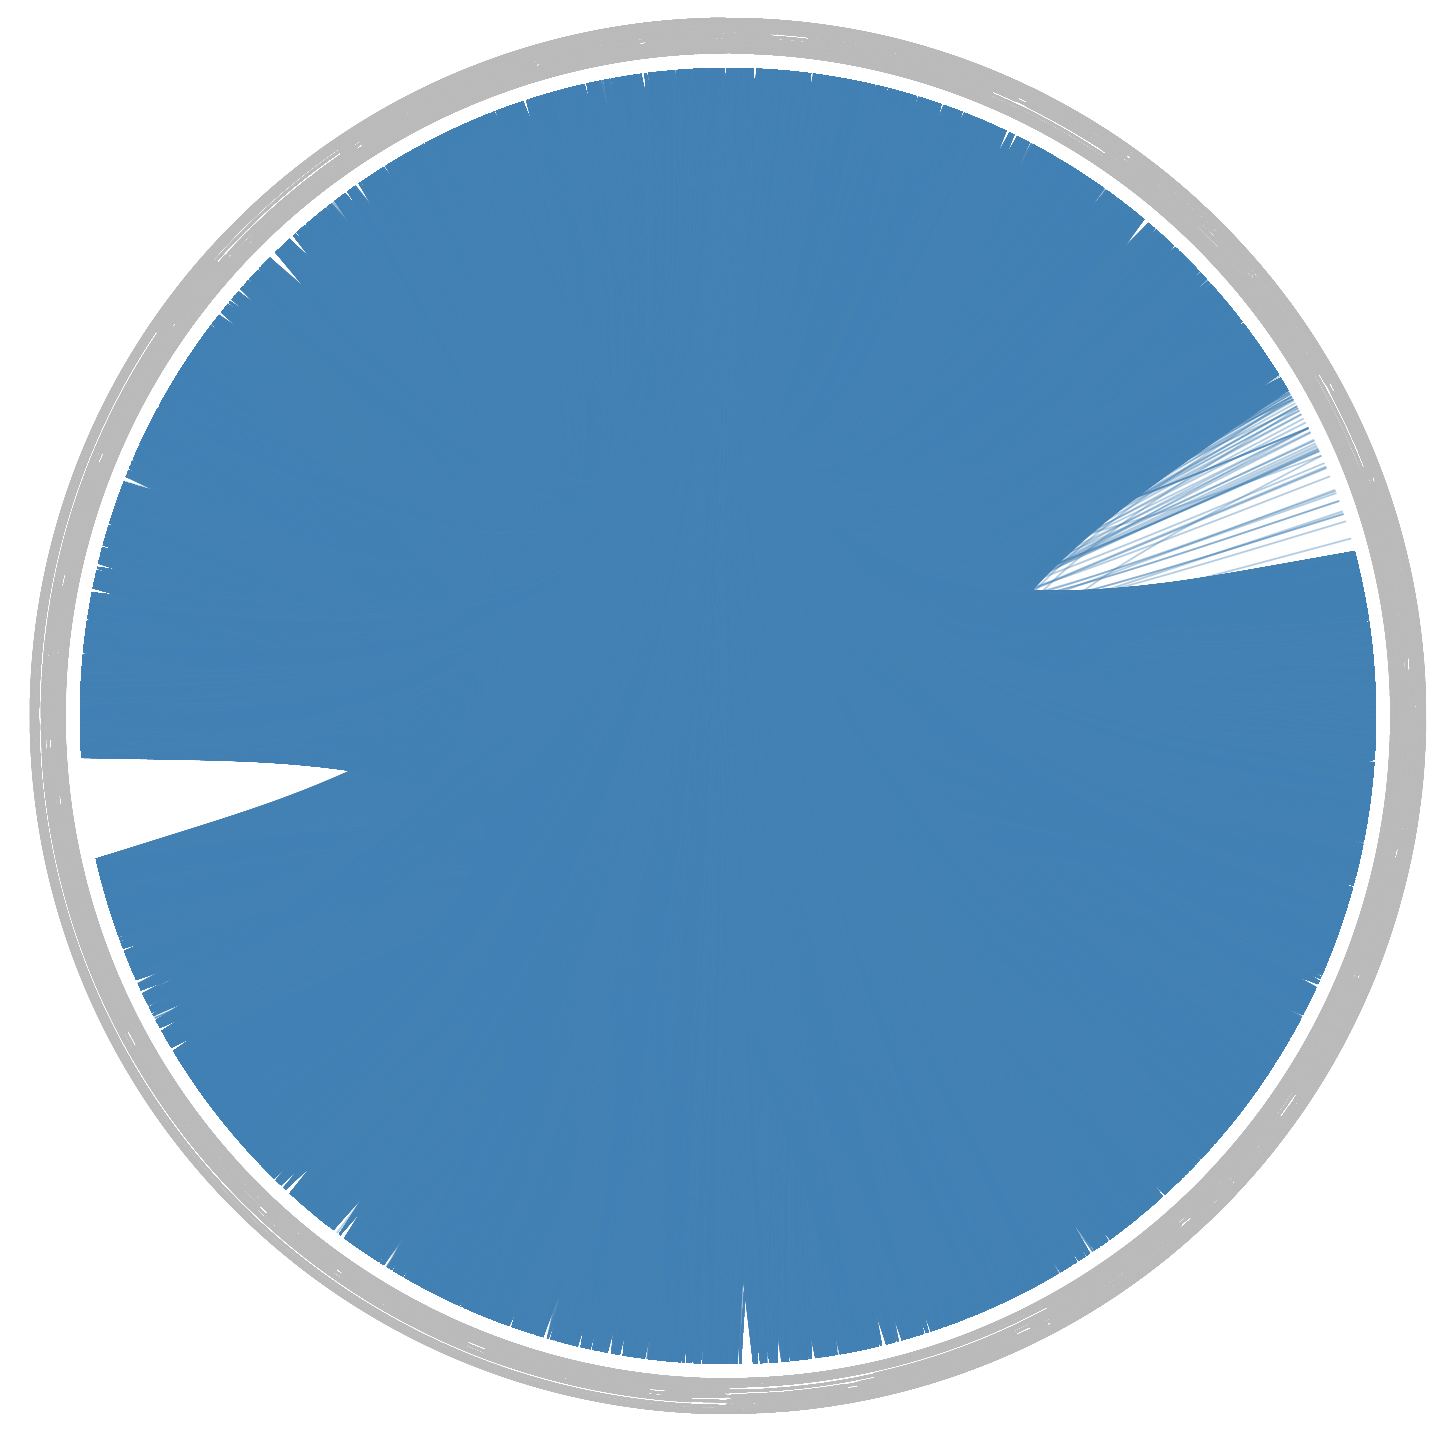
\includegraphics[scale=0.17]{after2}}
\caption{OEIS Theory Graph of Inferred Views using Method 2 \label{fig:after2}}
\end{subfigure}
\medskip
\small

The points around the circle represent the theories and the blue lines views between them. The theories presented
here are only the ones for which we have parsed the generating functions.

\caption{OEIS Theory Graphs}

\end{figure}

The relation finder is implemented in Scala and is available at \url{https://github.com/eluzhnica/ISFA}. The page
will be kept up to date with results. The implementation of the \emph{normalization} rules makes use of the parsing
tree of the expression that we get from the parsing phase. The \emph{transformations} are done using SageMath as a
math engine. Our Scala code communicates with a local SageMath server using a REST API. The SageMath calls are cached
 in Mongo for practicality during development.

Below, we walk through some examples of the relations found from each method.
\paragraph{Method 1}
This is more of a sanity check of the algorithm. Due to the nature of these relations, these are self-evident
relations. Additionally, these relations can be effectively searched utilizing a numerical method. An instance that
our algorithm finds is that sequence $A001478(n) = -A000012(n)$. Sequence $A001478$ is the sequence of the negative
integers, while $A000012$ is the sequence of positive integers.

\paragraph{Method 2}
An example of this method, which we have submitted and it is accepted in the \oeis (\url{https://oeis.org/A037532}),
is as follows.
Sequence $A037532$ has an ordinary generating function:
\begin{align}
\frac{x(1+x+2x^2)}{(x-1)(7x-1)(1+x+x^2)} \stackrel{\text{PFD}}{=} &\frac{1}{57}\frac{5x + 3}{x^2 + x + 1} -
\frac{\frac{29}{171}}{7x- 1} + \frac{\frac{2}{9}}{x - 1} \\
\stackrel{\text{Decomp.} + \rulename{Sort}}{=} &\frac{1}{57}\frac{5x}{1+x+x^2} + \frac{1}{57}\frac{3}{1+x+x^2} -
\frac{\frac{29}{171}}{-1 + 7x} + \frac{\frac{2}{9}}{-1 + x}
\end{align}
Sequence $A049347$:
\begin{equation}
\frac{1}{1+x+x^2}
\end{equation}
Sequence $A000420$:
\begin{equation}
\frac{1}{1-7x} \stackrel{\rulename{Sort}}{=} -\frac{1}{-1+7x}
\end{equation}
Sequence $A000012$:
\begin{equation}
\frac{1}{1-x} \stackrel{\rulename{Sort}}{=} -\frac{1}{-1+x}
\end{equation}

It is clear that the relation that can be derived here is:
\begin{equation} \label{eq:accepted}
A037532(n) = \frac{5}{57}A049347(n-1) + \frac{3}{57}A049347(n) + \frac{29}{171}A000420(n) - \frac{2}{9}
\end{equation}
There is one subtlety that needs to be explained. The sequence with ordinary generating function $\frac{1}{1-x}$ is
the sequence $(1,1,1, \ldots)$. However, for simplicity we write down $\frac{2}{9}$ instead of $\frac{2}{9}A000012(n)
$. However, our algorithm does not do that.

\paragraph{Method 3} An example relation is shown below.

Sequence $A257890$ has a generating function:
\begin{equation}
\frac{(x^2-x+1)(x^2-3x+3)}{(x-1)^6} = \frac{1}{(x - 1)^2} + \frac{1}{(x - 1)^4} + \frac{1}{(x - 1)^6}
\end{equation}
Sequence $A257199$ has a generating function:
\begin{align}
\frac{x(1 - x + x^2)}{(1 - x)^6} = \frac{1}{(x - 1)^3} + \frac{2}{(x - 1)^4} + \frac{2}{(x - 1)^5} + \frac{1}{(x - 1)
^6}
\end{align}

Clearly, $\frac{1}{(x-1)^6}$ is in common. But also, $-5\int \frac{1}{(x-1)^6} dx = \frac{1}{(x-1)^5}$, which makes
it possible to express a relation through $\frac{1}{(x-1)^5}$, too. In this case we can use the technique used in
Equation \ref{eq:transform} to carry over the relation to the representing functions since the representing functions
 of the corresponding sequences are known. Hence, we get the following relation:
\begin{multline}
A257890(n) = A000027(n+1) + A000292(n+1) \\
- \frac{n+1}{10}(A257199(n+1)
 + A000217(n+2) - 2*A000292(n+2) - A000389(n+6))
\end{multline}
Nonetheless, in the general case the relation cannot be always carried over to the representing function, so the
relation would only be in the level of the generating function.

Since our parser runs over all the formulas of \oeis, we have extracted the existing explicit relations in \oeis and
made a graph (Figure \ref{fig:before}) showing the existing connections between sequences .
The second method enriches the theory graph as shown in Figure \ref{fig:after2} and the third method as shown in
Figure \ref{fig:after}).

\begin{center}
 \begin{tabular}{||c | c||}
 \hline
 Parsed Generating Functions & 39\ 218 \\
 \hline
 SageMath syntax-proof Generating Functions & 22\ 757 \\
 \hline
 Verified Ordinary Generating Functions & 21\ 872 \\
 \hline
 Parsed Ordinary Generating Functions &  35\ 953 \\
 \hline
 SageMath verified Ordinary Generating Functions & 13\ 400 \\
 \hline
 Method 1 relations & 4\ 859 \\
 \hline
 Sequences in Method 1 relations & 853 \\
 \hline
 Method 2 relations & 262\ 751\ 850\\
 \hline
 Method 3 relations & 98\ 401 \\
 \hline
\end{tabular}
\end{center}

The number of parsed generating functions is self-explanatory. The generating functions are extracted from the formulae that were parsed during the parsing phase.
These generating functions are of all kinds - ordinary, Dirichlet, exponential generating functions 
just to name a few. However, we were only interested in the ordinary generating functions. 
Since the parser is not guaranteed to produce correct results, nor the filtering of the ordinary
generating functions, two verification methods are employed. The first verification method is used to filter the generating functions that we can compute on. The second verification method is used to 
filter the ordinary generating functions that are actually correct and that we can rely to generate
new relations. These are the generating functions that the relation-generation algorithms use. 
First, we translated the parsed generating functions in SageMath syntax and checked if they were accepted from SageMath. We name the generating functions that pass this test as 'SageMath syntax-proof Generating Functions' in the table above. From a manual inspection we notice that most of the generating functions that do not pass this test are due to external references to unknown functions. For instance, $1+Q(0)$ where the function $Q(n)$ is defined later on in the sequence document. Currently, we do not resolve these references.
Second, the parsed ordinary generating functions are used to generate the first 8 terms of the sequence and then matched against the first terms (fetched from \oeis). This is important to set a basis for correct relations. In fact, this is also
important to further verify the parsing accuracy aswell as the \oeis data. 
From an inspection of $70$ ordinary generating functions that failed the verification phase (data available at: \url{https://github.com/eluzhnica/oeis_gf/blob/master/failed}), only 1 was found to have been wrongly parsed. It was due to an unexpected mix of words and formulae.
On the other hand, from another (incomplete) inspection of the same data we noticed 18 incorrect generating functions in the \oeis.  Two of them were already fixed, we just had an older copy of the \oeis. The rest were mostly the generating function not matching the shift/initial terms. However, there was also a case where the generating function matched only the first 5 terms but not the rest. 
Finally, we also made a SageMath module where users can access the ordinary generating functions of the sequences and made it accessible at \url{https://github.com/eluzhnica/oeis_gf}.
% Most of the generating functions that are not qualified are due to  that were not being accepted were because they referred to some other functions. For
%   instance, $1+Q(0)$ where the function $Q(n)$ is defined later on in the sequence document. We currently do not
%   resolve these references.

Method 1 reports $4859$ relations of that kind. However, in total only $853$ sequences are involved in these relations.

One can notice that there is a plethora relations generated from the second method. However, this is expected.
Take for instance, $G = A + B + C + D$, where $G$ is the generating function of a sequence, and $A,B,C, D$ are the
partial fractions. If each partial fraction represents an \oeis sequence under every transformation (unit, derivate,
integrate), then the number of relations that we can form is actually $3^4$. Clearly,
the number of relations per generating function are bound by the exponential function $f(n) = 3^n$ where $n$ is the 
number of partial fractions (including the partial fractions that come from \emph{decomopose}). Since there are generating functions
with up to $22$ partial fractions, the big number of relations is not a big surprise.

Out of three relation submissions to the \oeis, two relations are already accepted
\cite{oeis-accepted-1,oeis-accepted-2} under the author's name. One of them has already
been presented in Equation \ref{eq:accepted} and the other relation is
$A001787(n) = A007283(n) \frac{n}{6}$ which can be found at
\url{https://oeis.org/A001787}. The unaccepted submission was not perceived to add new
information since a similar relation was already present. The submitted relations were
selected randomly.

%%% Local Variables:
%%% mode: latex
%%% TeX-master: "../report"
%%% End:
